\documentclass[xcolor=table]{beamer}

\mode<presentation> {
\usetheme{Madrid}
}

\usepackage{graphicx}
\usepackage[utf8]{inputenc} 
\usepackage[french]{babel}

\usepackage{multirow}
\usepackage[table]{xcolor}

\title{Authentification \`{a} base d'OTP}
\author{M1SSI}
\institute[Université de Rouen] {
Université de Rouen \\
\medskip
}
\date{\today}

\AtBeginSubsection[] 
{ 
\begin{frame}  
\frametitle{Plan} 
\tableofcontents[currentsubsection,hideothersubsections,subsectionstyle=show/shaded]
\end{frame}
} 

%------------------------------------------
\begin{document}

\begin{frame}
\titlepage
\end{frame}

\begin{frame}
\frametitle{Table des matières}
\tableofcontents
\end{frame}

%------------------------------------------------
\section{Introduction}
%------------------------------------------------

\begin{frame}
\frametitle{L'équipe}
\begin{block}{Le chef}
Adrien \bsc{Smondack}.
\end{block}
\begin{block}{La technique}
Yves \bsc{Adegoloye} et Damien \bsc{Picard}.
\end{block}
\begin{block}{La qualité}
Claire \bsc{Hardouin} et Gaëtan \bsc{Ferry}.
\end{block}
\begin{block}{La MOA}
Maxime \bsc{Michotte} et Benjamin \bsc{Zigh}.
\end{block}
\end{frame}


\begin{frame}
\frametitle{Le projet}

\begin{block}{Clients}
\begin{description}
\item[Magali \bsc{Bardet}:] Enseignante-Chercheuse à l'université de Rouen.\\
\item[Bruno \bsc{Macadré}:] Ingénieur Système à l'université de Rouen.
\end{description}
\end{block}

\begin{block}{Sujet}
Création d'un système d'authentification à base de mots de passe jetables.
\end{block}
\end{frame}




%------------------------------------------------
\section{Concepts fondamentaux}
%------------------------------------------------
\subsection{L'authentification}
\begin{frame}
\frametitle{Authentification}
\begin{block}{Principe de base}
L'utilisation d'une empreinte produite à partir d'un facteur, permettant d'identifier un utilisateur.
\end{block}
\begin{block}{Les types de facteurs}
\begin{description}
\item[Mémoriel:] Mot de passe, phrase de passe...
\item[Matériel:] Clé USB, certificat numérique, carte à puce...
\item[Corporel:] Empreinte digitale, pupille, voix...
\item[Réactionnel:] Signature, challenge...
\end{description}
\end{block}
\end{frame}


\subsection{L'authentification classique}
\begin{frame}
\frametitle{Principe de base}
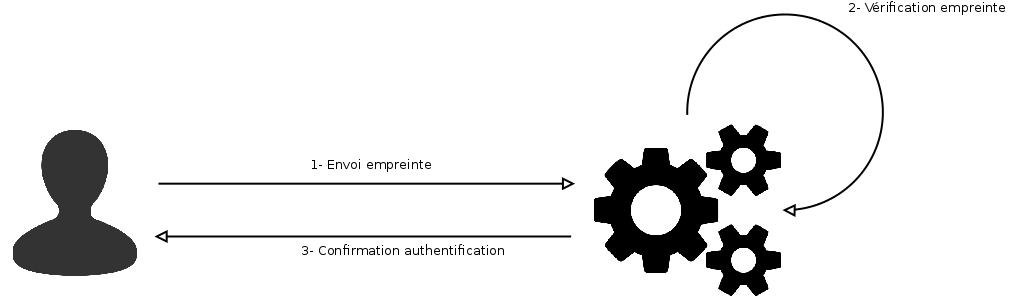
\includegraphics[scale=0.24]{../graphics/authsimple.png}
\end{frame}

\begin{frame}
\frametitle{Exemple}
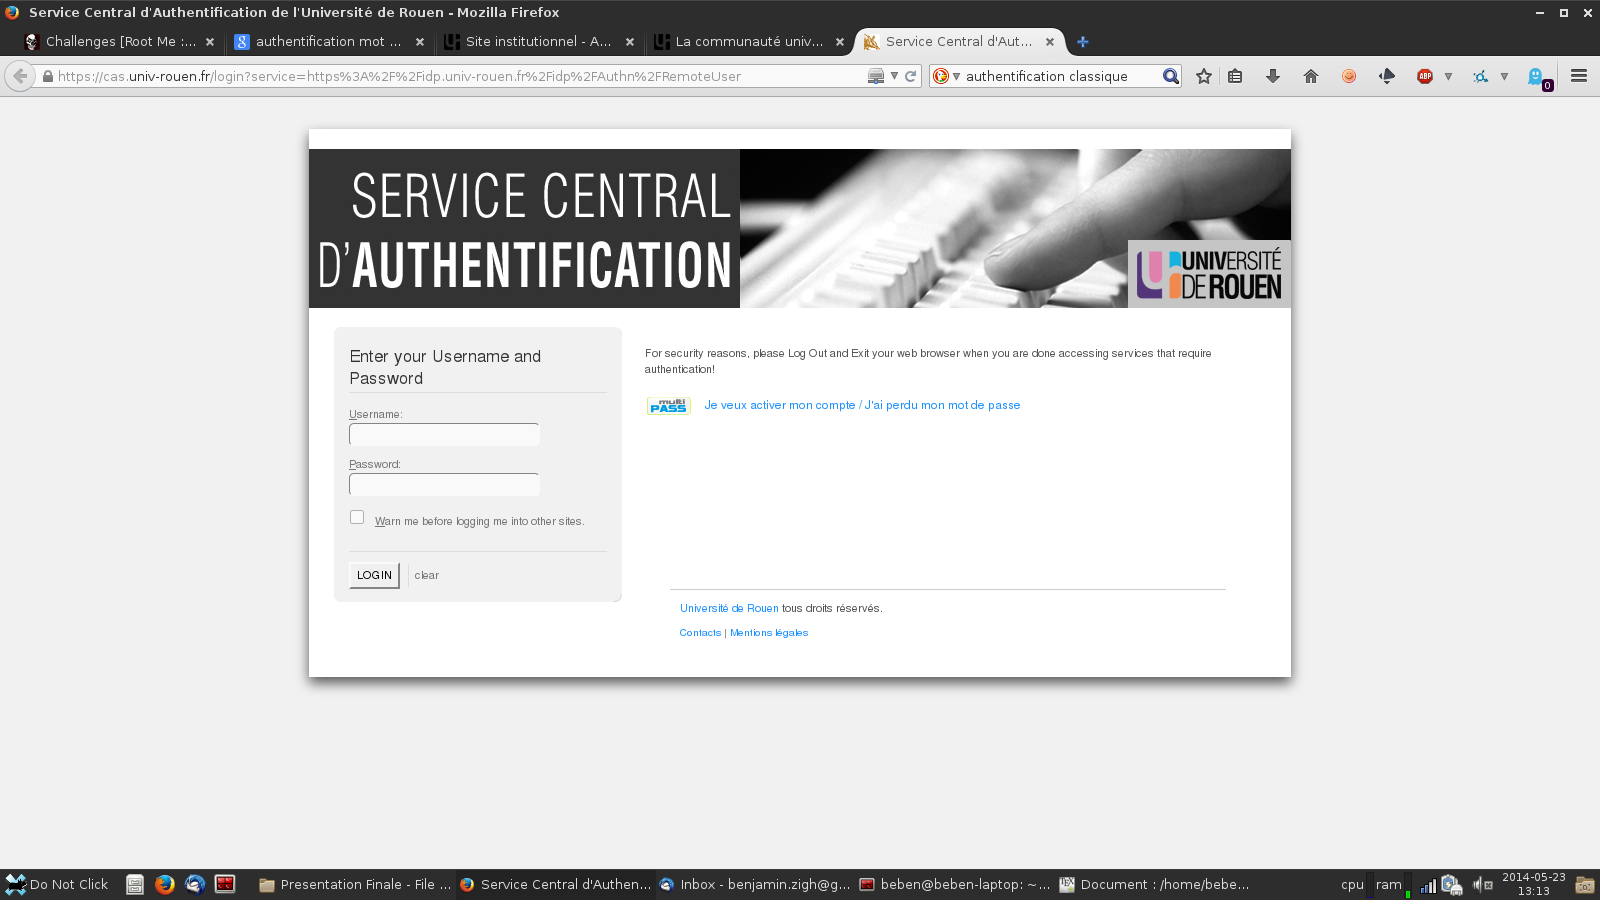
\includegraphics[scale=0.21]{../graphics/auth-mdp.png}
\end{frame}



\subsection{L'authentification par OTP}

\begin{frame}
\frametitle{Principe}
\begin{block}{Définition}
    Un OTP est un mot de passe jetable, c'est à dire qu'il satisfait les deux 
  critères suivants:
  \begin{itemize}
    \item Il n'est pas prévisible
    \item Il n'est valide que pour une unique session.
  \end{itemize}
\end{block}

\begin{block}{Utilité}
  \begin{itemize}
    \item Permettre une authentification à 2 facteurs (forte).
    \item Éviter les attaques par rejeu.
  \end{itemize}
\end{block}
\end{frame}

\begin{frame}
\frametitle{Exemples}
\begin{center}
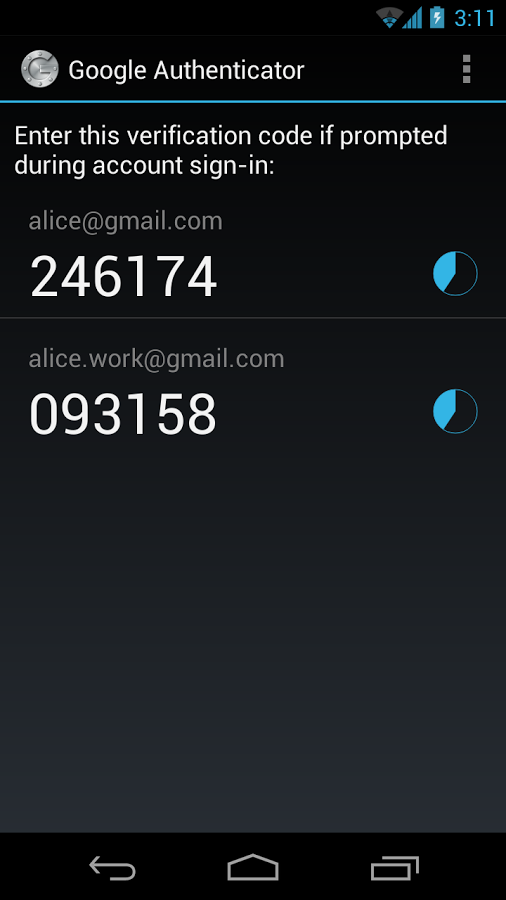
\includegraphics[scale=0.2]{../graphics/googleauth.png}
\hspace{1em}
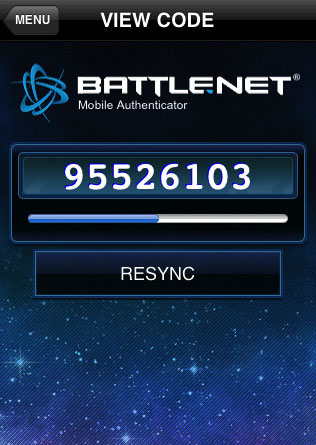
\includegraphics[scale=0.405]{../graphics/blizzardauth.jpg}
\end{center}


\end{frame}

\subsection{L'authentification cryptographique}
\begin{frame}
\frametitle{Principe}
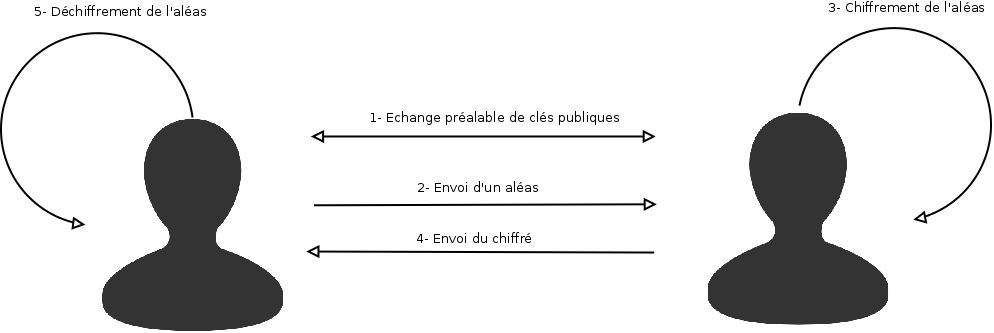
\includegraphics[scale=0.24]{../graphics/authcrypt.png}
\end{frame}

\begin{frame}
\frametitle{Utilisation}
\begin{block}{SSH}
Il est possible de se connecter via SSH en employant des clés RSA.
\end{block}

\begin{block}{HTTPS}
Les clés publiques, gérées par des PKIs\footnote{Public Key Infrastructures}, sont utilisées pour authentifier les serveurs de façon sécurisée sur internet.
\end{block}
\end{frame}

\subsection{Récapitulatif}
\begin{frame}
\frametitle{Récapitulatif}
%\begin{center}
%\begin{tabular}{|c|c|c|c|}
%\hline
%  & Classique & OTP & Crypto \\ \hline
%Rejeu & O & N & N \\ \hline
%MITM & O& O& N\\ \hline
%\end{tabular}
%\end{center}
\begin{block}{Classique}
Vulnérable aux attaques par rejeu et aux attaques de type MITM\footnote{Man In The Middle}.
\end{block}

\begin{block}{OTP}
Protégé contre les attaques par rejeu.
\end{block}

\begin{block}{Cryptographique}
Protégée contre les attaques par rejeu et MITM.
\end{block}

\end{frame}


\section{La mise en œuvre}

\subsection{Demande du client}

\begin{frame}
\frametitle{Le livrable 1/2}
\begin{block}{État de l'art} 
Un état de l'art comprenant au moins trois protocoles OTP étudiés.
\begin{description}
 \item[OTP] Protocole de base.
 \item[HOTP] Protocole utilisant la fonction HMAC et un compteur de 
  synchronisation.
 \item[TOTP] Protocole reprenant HOTP avec le temps comme compteur.
 \item[EAP-POTP] Architecture pour s'authentifier sur \verb?IEEE 802.1x?. 
 \item[OTPW] Protocole basé sur l'état de la machine et la fonction de hachage RipeMD-160.
\end{description}
\end{block}
\end{frame}

\begin{frame}
\frametitle{Le livrable 2/2}
\begin{block}{Application}
    L'application se ferait sur les protocole qui auraient été retenus après l'étude de 
  l'état de l'art et comporterait pour chaque protocole:
  \begin{itemize}
    \item Un module d'authentification.
    \item Un token\footnote[1]{Programme permettant à l'utilisateur d'obtenir un 
      OTP pour s'authentifier.}
  \end{itemize}
\end{block}

\end{frame}

%------------------------------------------------
\subsection{L'état de l'art}
%------------------------------------------------
\begin{frame}
\frametitle{Formation des équipes de travail}
\begin{block}{Équipes de recherche}
  \begin{itemize}
    \item EAP-POTP
    \begin{itemize}
      \item Tayewo-John-Yves \bsc{Adegoloye}
      \item Claire \bsc{Hardouin}
    \end{itemize}
    \item HOTP - TOTP
    \begin{itemize}
      \item Gaëtan \bsc{Ferry}
      \item Maxime \bsc{Michotte}
      \item Benjamin \bsc{Zigh}
    \end{itemize}
    \item OTPW - OTP
    \begin{itemize}
      \item Damien \bsc{Picard}
      \item Adrien \bsc{Smondack}
    \end{itemize}
  \end{itemize}
\end{block}
\end{frame}

\begin{frame}
\frametitle{La méthode}
\begin{block}{Le canevas}
\begin{itemize}
\item Mis en place par le responsable qualité.
\item Un squelette de document TeX à remplir.
\item Contient les questions à poser pour chaque technologie.
\end{itemize}
\end{block}
\begin{block}{Présentations}
\begin{itemize}
\item Avant la compilation des trois en un rapport.
\item Chaque équipe explique aux deux autres sa partie.
\end{itemize}
\end{block}
\end{frame}

\begin{frame}
\frametitle{Le bilan: OTP}
\begin{block}{HOTP}
\begin{itemize}
\item Basé sur HMAC\footnote{Hashed Message Authentication Code}.
\item Plus facile à utiliser pour le client.
\end{itemize}
\end{block}

\begin{block}{TOTP}
\begin{itemize}
\item Basé sur HOTP, emploie HMAC.
\item Le standard de l'industrie, employé par la plupart des méthodes OTP grand public.
\end{itemize}

\end{block}
\end{frame}


\begin{frame}
\frametitle{Le bilan: livrables}
\begin{block}{Module PAM}
\begin{itemize}
\item Facilité d'installation sur de nombreux systèmes (Linux, SSH, Apache...).
\item Compatibilité avec les authentifications existantes.
\end{itemize}
\end{block}

\begin{block}{App Android}
\begin{itemize}
\item Grande réserve d'utilisateurs.
\item Facilement transportable.
\item Système \og libre \fg{}. 
\end{itemize}
\end{block} 
\end{frame}

\begin{frame}
\begin{center}
\Huge{Démonstration}
\end{center}
\end{frame}


%------------------------------------------------
\subsection{Organisation du développement}
%------------------------------------------------

\begin{frame}
\frametitle{Méthodologie}
\begin{center}
\Huge Agile (adapté)
\normalsize
\begin{block}{Les grands principes}
\begin{itemize}
 \item Test Driven Development (XP).
 \item Intégration continue et Refactoring (XP).
 \item Appropriation collective du code (XP).
 \item Réunions client régulières et adaptabilité.
 \item Réunions d'équipe régulières.
\end{itemize}
\end{block}
\end{center}

\end{frame}

\begin{frame}
\frametitle{Répartition}
\begin{block}{Équipes de développement}
  \begin{itemize}
    \item Module PAM
    \begin{itemize}
      \item Claire \bsc{Hardouin}
      \item Damien \bsc{Picard}
      \item Adrien \bsc{Smondack}
      \item Maxime \bsc{Michotte}
    \end{itemize}
    \item App Android
    \begin{itemize}
      \item Gaëtan \bsc{Ferry}
      \item Benjamin \bsc{Zigh}
      \item Tayewo-John-Yves \bsc{Adegoloye}
    \end{itemize}
  \end{itemize}
\end{block}
\end{frame}




%------------------------------------------------
\subsection{Aspect technique}
%------------------------------------------------

\begin{frame}
\frametitle{Technologies utilisées}
\begin{block}{Systèmes d'exploitation}
\begin{itemize}
\item GNU/Linux pour le module d'authentification.
\item Android pour le token.
\end{itemize}

\end{block}
\begin{block}{Langages}
\begin{itemize}
  \item Pour le module PAM, le C est obligatoire.
  \item Pour le token Android, Java est recommandé. 
\end{itemize}
\end{block}
\end{frame}


\begin{frame}
  \frametitle{Tests et vérifications}
  \begin{itemize}
   \item Procédures de tests écrites au début du développement de chaque composante. (Test Driven Development)
   \item Tests exécutés par les équipes de développement tout au long du processus de création.
   \item  Lorsque des anomalies sont détectées lors des tests, la procédure est la suivante:
    \begin{itemize}
     \item Création d'une note / mémo précisant l'anomalie rencontrée.
     \item Ajout d'une entrée au journal de test précisant la date du test.
     \item Diffusion de la note à l'équipe de développement pour correction.
    \end{itemize}
  \end{itemize}
\end{frame}




\subsection{Le module PAM}
\begin{frame}
\frametitle{PAM: Architecture logicielle}
\begin{figure}
 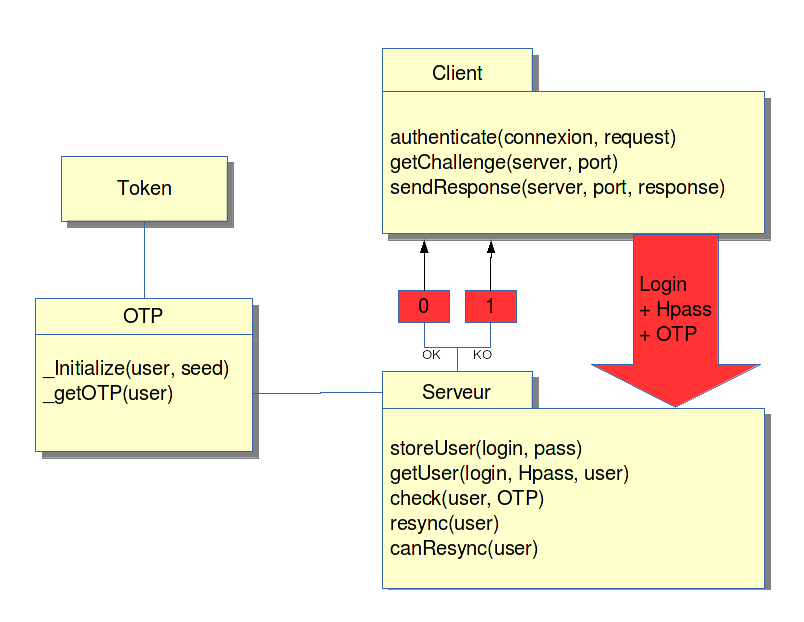
\includegraphics[scale=0.3]{../graphics/architecture.png} 
 \caption{Schéma de l'architecture logicielle}
\end{figure}

\end{frame}
\begin{frame}
\frametitle{Gestion de secrets}
Développement d'une bibliothèque chargée de la représentation des secrets en mémoire.
\begin{itemize}
  \item Structure en mémoire.
  \item Gestion de ressources mémoire.
  \item Création aléatoire.
  \item Création à partir d'une entrée utilisateur.
  \item Représentation dans différente bases.
\end{itemize}

Permet de faciliter la gestion de la mémoire.
\end{frame}

\begin{frame}
\frametitle{Génération de mots de passe jetable}
développement d'une bibliothèque permettant de générer des mots de passe selon un secret
et un compteur.
\begin{itemize}
\item Permet de générer selon les méthodes HOTP et TOTP.
\item Implémentation respectant la RFC 4226.
\item Repose sur la bibliothèque de gestion des secrets.
\end{itemize}

\end{frame}

\begin{frame}  
\frametitle{Gestion des utilisateurs}
Bibliothèque permettant d'enregistrer les utilisateur dans un fichier.
\begin{itemize}
  \item Structure en mémoire.
  \item Enregistrement.
  \item Lecture.
  \item Gestion ressources en mémoire.
\end{itemize}

Niveau d'abstraction supplémentaire.
\end{frame}

\begin{frame}
\frametitle{L'interface de programmation pour module PAM}
\begin{itemize}
  \item Un module est écrit en langage C.
  \item Doit implémenter une ou plusieurs fonctions correspondant chacune à une fonctionnalités.
  \item Doit être compilé comme une bibliothèque partagée.
  \item L'interface de programmation permet d'interagir avec l'utilisateur.
\end{itemize}

\end{frame}

\begin{frame}
\frametitle{Développement du mécanisme d'authentification}
\begin{itemize}
\item Implémentation de la fonction \verb?pam\_sm\_authenticate? dans le module.
\item Repose sur les bibliothèque de génération de mots de passe jetable et de gestion
des utilisateurs.
\item Implémente les mécaniques de vérification de mots de passe jetable et de resynchronisation.
\end{itemize}
\end{frame}

\begin{frame}
\frametitle{Gestion de la mise à jour des données utilisateurs}
\begin{itemize}
  \item Implémentation de la fonction \verb?pam\_sm\_chauthtok? dans le module.
  \item Repose sur le mécanisme d'authentification et les bibliothèques de gestion
  d'utilisateurs et de secrets.
  \item Facilite la création de secrets pour les utilisateurs.
  \item Accessible via un utilitaire en ligne de commande.
\end{itemize}

\end{frame}



\subsection{L'app Android}
\begin{frame}
\frametitle{Android: Architecture logicielle}
\begin{figure}
 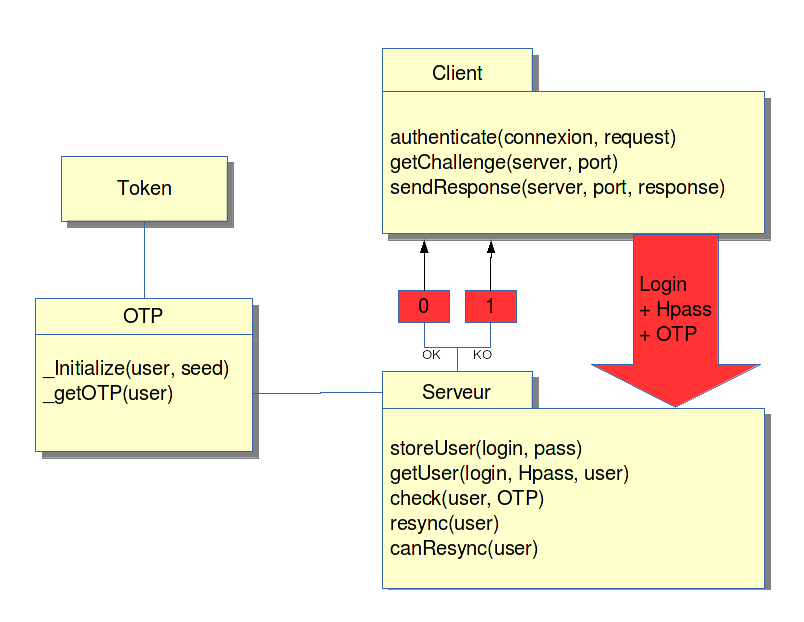
\includegraphics[scale=0.3]{../graphics/architecture.png} 
 \caption{Schéma de l'architecture logicielle}
\end{figure}

\end{frame}

\begin{frame}
\frametitle{Compatibilité}

\end{frame}
\begin{frame}
\frametitle{Bibliothèque OTP}
\end{frame}

\begin{frame}
\frametitle{Sécurité des données}

\end{frame}

\begin{frame}
\frametitle{Interface Utilisateur}
\end{frame}

\begin{frame}
\frametitle{Synchronisation d'horloge}
\end{frame}

\subsection{Licence}
\begin{frame}
\frametitle{Les différentes licences}

\end{frame}

\begin{frame}
\frametitle{La licence choisie}

\end{frame}

%------------------------------------------------
\section{Conclusion}
%------------------------------------------------
\begin{frame}  
\frametitle{Plan} 
\tableofcontents[currentsection,hideothersubsections]
\end{frame}

\begin{frame}
\frametitle{Résultat des tests finaux}

\end{frame}

\begin{frame}
\frametitle{Enseignements tirés du projet}

\end{frame}


\begin{frame}
\frametitle{Améliorations possibles}
\end{frame}

\begin{frame}
\frametitle{Conclusion}
\begin{itemize}
\item Un projet dans l'ère du temps.
\item Un panel de connaissances variées.
\item Une première expérience de gestion de projet.
\end{itemize}
\end{frame}




%------------------------------------------------
\end{document}